\chapter{Result and Evaluation}
\label{chap:Evaluation}
\index{Results and Evaluation}

%%%%%%%%%%%%%%%%%%%%%%%%%%%%%%%%%%%%%%%%%%%%%%%%%%%%%%%%%%%%%%%%%%%%%%%%%%%%%%%%
%In this chapter, we describe the method we used to evaluate our solution
%and report the result we obtain from the evaluation process.
%For the person ReID task we will use two most popular metrics acknowledged by
%the
%research community to evaluate our work.
%For the framework part we are going to evaluate our implementation according
%to
%the goal,
%requirement and usage scenarios we defined in \autoref{sec:intro-mot-goal} and
%\autoref{sec:intro-scen-req}.

In this chapter, we will first evaluate our framework solution to show that we
achieve the goal we set up at the very beginning in \autoref{sec:intro-mot-goal}
and both the functional and non-functional requirements listed in
\autoref{sec:intro-scen-req} are fulfilled as well as the scenarios are
realized by the application we described in \autoref{chap:fw-app}.
After demonstrating we can achieve the goal, we also would like to tell how
well we can do it. So we describe the common metrics which are acknowledged by
the corresponding research community. Then we employ exactly the same approach
to evaluate our algorithms (or models) and report our result respect to these
metrics.

\section{Framework Evaluation}
\label{sec:Eval-framework}

We proposed a framework approach in \autoref{chap:fw-design} to address the
limitation we mention in \autoref{sec:intro-lim-issv2} and listed both the
functional and non-functional requirements in \autoref{sec:intro-scen-req}.
%In the previous section, we have already shown the evaluation result for the algorithms
%(or models) used for person detection and person recognition problems.
%In this section, we are going to demonstrate the advantages of our framework
%solution and shown that this approach makes it more valuable than just solve it
%by a piece of program.
In this section, we will examine the requirements and scenarios one by one to show
how our solution addresses them. Also, we are going to demonstrate the advantages
of our framework solution and show that this approach makes it more valuable and
interesting than just solve it by a piece of program.

%\subsection{Realization of Scenarios}
%\label{sec:Eval-scenarios}
%In \autoref{sec:intro-scen-req}, we give a list of usage scenarios of our
%solution
%and extract the functional requirements from these scenarios. In this section,
%we will walk through them and show that they can be realized well by employing
%the proposed framework method.

\subsection{Device Switch and New Device Addition}
\label{sec:Eval-framework-device}

As mentioned in \autoref{sec:fw-inst-device}, we have a device module that
provide
the abstraction of various physical devices for the framework that would enable
the switch among various devices easily and also will not increase the
complexity a lot of adding a new device.

\textbf{Device switch:}  For both Kinect and RealSense cameras we provide a
minimum working sample code for the users to see how to use it (as a starting
point). These code can be found under the path
\texttt{sample/kinect/kinect\_capture.cpp} and
\texttt{sample/rs435/rs\_capture.cpp}. From these two files, we can find that
the only differences between them are just one line code (even we can say
just one word changed to switch between Kinect and RealSense), shown by
\autoref{fig:fw-device-diff}. It clearly demonstrated that our solution
fulfill \textbf{FR1} proposed in \autoref{sec:intro-sq-dev}.

\begin{figure}
    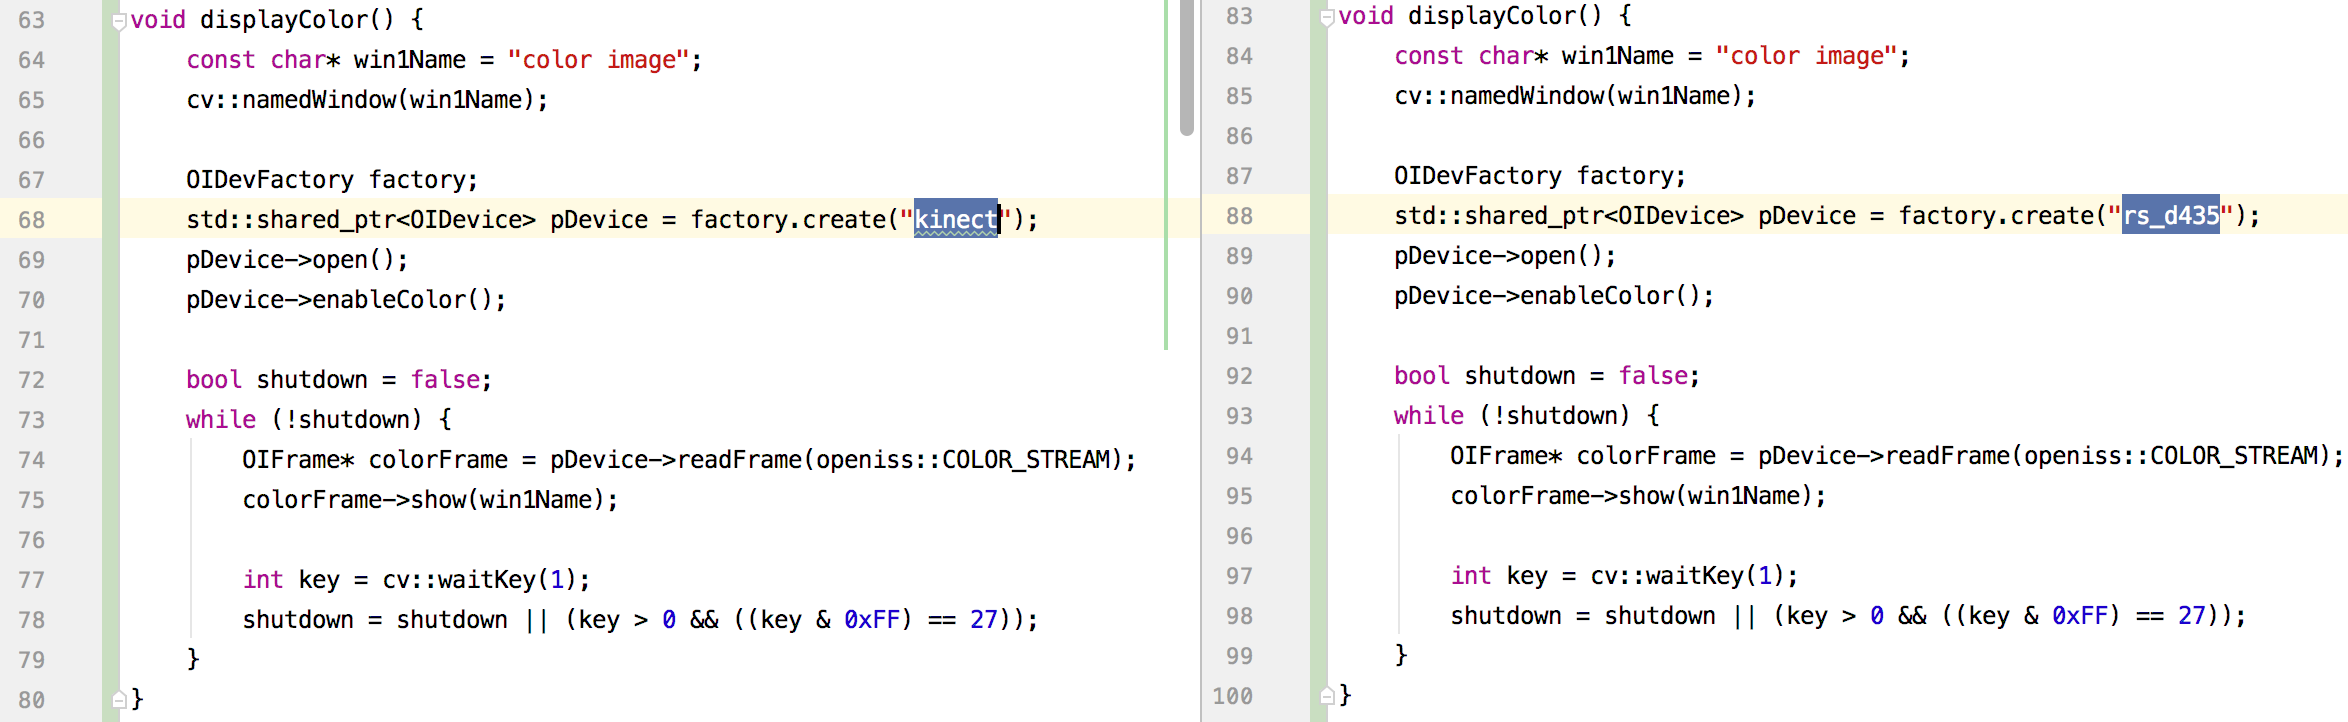
\includegraphics[width=\linewidth]{figures/framework_device_diff.png}
    \caption[Effort needed to switch between different cameras]
    {Effort needed to switch between different cameras, left is code for Kinect
        and right is the code with same effect for RealSense.}
    \label{fig:fw-device-diff}
\end{figure}

\textbf{New device addition:} Since we have an abstraction layer on top of each
concrete device implementation, we have to admit that when we try to add a new
device it will introduce a little bit more work compared to we don't have any
abstraction. But if we look at the convenience (one word changed for adding new
device) it brings to us we believe everyone agrees it is necessary. Under our
design of the framework, you will need to following steps to add a new device.
It is evidence which can clearly demonstrate that we fulfill
\textbf{FR2} proposed in \autoref{sec:intro-sq-dev}.

\begin{enumerate}
    \item Create a new class inherited from \texttt{OIDevice} and implement all
    its pure virtual methods under the directory \texttt{src/}.

    \item Since we employed the factory design pattern, you still need to add
    the logic to instantiate the appended device in \texttt{OIDeviceFactory}
    class as well as the device-related memory deallocation when it is useless.
\end{enumerate}

\subsection{Back-end Abstraction}
\label{sec:Eval-framework-backend}

As explain in \autoref{sec:intro-mot-goal}, we want the OpenISS framework can
serve
as a back-end of our previous work ISSv2. The image alignment application we
introduced in \autoref{sec:Impl-fw-app-align} is a good showcase for it. In this
application,  no matter what kinds of camera you are using,
the low-level APIs like \texttt{OIDevice} abstract the physical
device providing the operands (e.g. intrinsic, extrinsic matrices and the data
for each frame) needed for the image alignment computation. Then the aligned
frame will be encapsulated as an OpenISS data structure \texttt{OIDataFrame}
and return to the user.
These processes, abstraction and encapsulation, are the core ideas of a
back-end system which provides a set of usable and convenient unified APIs for
the front-end to request without worrying about the complexity and
implementation details. The same applies to other applications mentioned in
\autoref{sec:Impl-fw-app-other}, they all proved that the back-end abstraction
is properly implemented and usable which means the requirements are
conceptually satisfied.
But we have to admit that one more step needs to be done to
complete the back-end abstraction. Since the ISSv2 was developed in Java and
our current solution is written in C/C++. A Java wrapper that can expose the
functionalities from our framework to ISSv2 is still missing.

\subsection{Person Re-identification and Skeleton Tracking}
\label{sec:Eval-framework-reid-skt}

In \autoref{sec:intro-sq-reid} and \autoref{sec:intro-sq-skt}, we stated the
scenarios of person re-identification and skeleton tracking. From these two
scenarios, we extracted requirements related to these two functionalities.
In \autoref{sec:fw-design-spec}, we described the design of our framework
solution showing its ability to address the ReID and tracking tasks in general.
In \autoref{sec:fw-inst-detector}, \autoref{sec:fw-inst-recoginzer} and
\autoref{sec:fw-inst-tracker} we described an instance of our framework which
provides the functionalities that can solve our specific problem. In
\autoref{sec:fw-app-reid} and \autoref{sec:fw-app-skt}, we described the
application built on top of our framework demonstrating how we use our solution
to solve our specific ReID and skeleton tracking problems.

The ReID application which described in \autoref{sec:fw-app-reid} clearly
demonstrated that it can detect the appearance of pedestrian and recognize that
found particular identity among a pre-defined database, which exactly fulfill
\textbf{FR4} and \textbf{FR5} proposed in \autoref{sec:intro-sq-reid}.

The skeleton tracking application which described in \autoref{sec:fw-app-skt}
clearly demonstrated that it can detect the appearance of pedestrian and
extract their skeleton points then keep tracking of them which exactly fulfill
\textbf{FR6} proposed in \autoref{sec:intro-sq-reid}.

\subsection{Extensibility}
\label{sec:Eval-framework-ext}

In \autoref{sec:intro-non-func-req}, by analyzing the usage scenarios described
in \autoref{sec:intro-scen-req}. We noticed that our solution should have
extensibility as its non-functional requirement.
The device switch and new device addition which we just explained in
\autoref{sec:Eval-framework-device} is actually a good showcase for it.
Also, our skeleton tracker instance is another case. As explain in
\autoref{sec:fw-inst-tracker}, we have a set of frozen spot defined for skeleton
tracking, they are \texttt{OITracker}, \texttt{OITrackerFrame},
\texttt{OIUser}, \texttt{OIUserMap} and \texttt{OISkeleton}. When we want
integrate an existing tracker or develop a new one, the work will be just to
create the corresponding hot spots, the process can be described as following:

\begin{enumerate}
    \item Create a concrete subclass inherited from \texttt{OITracker} and
    implement all the pure virtual methods.

    \item Create a subclass of \texttt{OITrackerFrame} which is the wrapper of
    the data holder classes mentioned above, link it to \texttt{OITracker} class
    within its \texttt{readFrame} function.

    \item Implement the logic for skeleton tracking algorithm for each coming
    image in the function named    \texttt{update} in \texttt{OITrackerFrame}.

    \item Add a new string as name to indicate the appended tracker and create
    an entry of it in the \texttt{OITrackerFactory} class.
\end{enumerate}

What's more, the cross-language module and pipeline module are also showcases
for extensibility. For the cross-language module, the way to add a new Python
model (can be implemented with any Python-based deep learning framework) or any
Python code-base can be described below:

\begin{enumerate}
    \item Make a copy of your existing Python script, let's say with name
    ``example.py", and all its dependencies into \texttt{project\_root/python/}
    folder and assume the function we want to expose named ``\texttt{func}".
    \item Create a C++ wrapper class under \texttt{project\_root/src/}
    directory, the wrapper class should have a member variable with type
    \texttt{OIPythonEnv} initialized by the file name (example.py) and target
    function name (\texttt{func}). Then create a corresponding wrapper
    function, let's say call ``\texttt{wrapper\_func}", for the Python function
    ``\texttt{func}".
    \item Create helper functions to pack the parameter(s) and unpack the
    return value if needed.
    \item In the application code, create an instance of the wrapper class,
    use ``\texttt{wrapper\_func}" as ``\texttt{func}".
\end{enumerate}

For the pipeline module, the extensibility is reflected by the
\texttt{OIFlowable} interface. Any class which can act or be expected to act as
a filter (really common in a computer vision framework) can implement it then
being pushed into a pipeline instance.
It is independent from any other modules in the core or specialized framework
which means it will not have any side effect on the existing implementation but
just extend them.
In order to create a new \texttt{OIFlowable} instance, you have to agree with
interface providing concrete implementation of all abstract methods and create
a compatible instance of \texttt{OIFlowContext} to work with it.
Further more, with the pipeline module, the flow of control become more 
predictable. It means the framework have larger power to hack into each step
providing more useful functionality. For example, if we have 10 kinds of 
person recognition algorithms and would like to know the time consuming by each 
of those in order to select the fastest one. Then we can put two timer filters 
right next to the recognizer without changing the code of the recognizer itself.
That's perfectly fit to the concept of OCP (open-closed principle) which means 
that software entities should open for extension ,but close for modification. 

\subsection{Usability}
\label{sec:Eval-framework-usab}
% what it can do
% can do it with ease

From \autoref{sec:intro-non-func-req}, usability is also one of the
non-functional requirement of our solution. It requires the software we
provided can at least achieve the goal we set up at the beginning, then further
it should also be easy to use from the user point of view.

To prove our framework is actually usable, in \autoref{chap:fw-app}, we
listed all the sample applications we provided along with our framework.
These applications can serve as proof clearly show that our framework can
be used to perform the following tasks:

\begin{itemize}
    \item Capture data from various physical devices and display them.
    \item Use the captured data to perform person detection in real-time.
    \item Use the person detection result and pre-defined database to achieve
          real-time person re-identification.
    \item Calibrate the connected camera sensors.
    \item Align the captured depth image to the corresponding color image.
    \item Remove background for a captured image specified by a distance
          threshold.
    \item Allow C/C++ code to communicate with Python code
    \item Allow the user to assemble different filters for various kinds of
          task flexibly.
\end{itemize}

To demonstrate our framework can be used with ease, the minimum example we
mention in \autoref{sec:Eval-framework-device} shows that just 14 lines of code
we can activate the device accessing the data and display them. Also from the
pedestrian detector sample code \texttt{sample/yolo/main.cpp}, we found
that to enable the whole person detection pipeline and display the result just
takes 18 lines of code. What's more, for the ReID pipeline, just 36 lines of
code we can query data from a device, perform the detection and re-identification
as well as comparison with the database and display the result. Last but not
least, for advanced users who may want to integrate their custom deep learning
model the procedure is also straight forward. With our cross-language invocation
module, all you need to do just create a wrapper class then specified your
Python script name and the functions you would like to expose, the person
detection and person recognition described in \autoref{sec:fw-inst-detector}
and \autoref{sec:fw-inst-recoginzer} respectively are good showcases of it.



\section{Person Re-identification Evaluation}
\label{sec:Eval-reid-app}

Recap what we discuss in \autoref{sec:intro-pbstat}, person ReID task can be
divided into three subtasks: person detection, person tracking and
person retrieval. In our solution, we have omitted person tracking
since we performed detection on each incoming frame which has the
same effect as tracking. The way used to evaluate detection and
retrieval algorithms have already been well-defined and acknowledged
within the community. In this section, we will introduce these
evaluation methods and report the result we obtained based on our
implementation.

Before we move to the evaluation methods, we give detail of the
environment setting we are using both for training and testing.
There is a total of two environments we have one is a local desktop machine
and the other is the Virya cluster provided by the faculty. The hardware
specification of these two environments shown as
\autoref{tab:eval-env-hardware}. We will refer them as \texttt{setting 1}
and \texttt{setting 2} respectively in the following content. There is a slight
difference between the software version installed in these two environments
shown as
\autoref{tab:eval-env-software}.

\begin{table}[]
    \centering
    \resizebox{\textwidth}{!}{%
    \begin{tabular}{|l|l|c|l|}
        \hline
        \multicolumn{1}{|c|}{\textbf{Setting}} &
        \multicolumn{1}{c|}{\textbf{Name}} & \textbf{Amount} &
        \multicolumn{1}{c|}{\textbf{Device}} \\ \hline
        \multirow{4}{*}{1(Desktop Machine)} & Memory & 1 & 7.7 GB \\ \cline{2-4}
        & Processor & 1 & Intel Core i5-3470 CPU @3.20GHz $\times$ 4 \\
        \cline{2-4}
        & Graphics & 1 & GeForce GTX 1070 Ti (8GB memory) \\ \cline{2-4}
        & OS & N/A & Ubuntu 18.04.1 LTS 64-bit \\ \hline
        \multirow{4}{*}{2 (Virya Cluster)} & Memory & 1 & 400 GB \\ \cline{2-4}
        & Processor & 1 & 72-core CPU \\ \cline{2-4}
        & Graphics & 8 & Tesla V100 (32 GB memory) \\ \cline{2-4}
        & OS & N/A & Scientific Linux \\ \hline
    \end{tabular}%
    }
    \caption{Environment hardware specification.}
    \label{tab:eval-env-hardware}
\end{table}

\begin{table}[]
    \centering
    \begin{tabular}{|r|c|c|}
        \hline
        \multicolumn{1}{|c|}{\textbf{Software}} &
        \multicolumn{1}{c|}{\textbf{Setting 1}} &
        \multicolumn{1}{c|}{\textbf{Setting 2}} \\ \hline
        Python & 3.6.7 & 3.6.8 \\ \hline
        TensorFlow & 1.12.0 & 1.13.1 \\ \hline
        Keras & 2.2.4 & 2.2.4 \\ \hline
        Keras-application & 1.0.6 & 1.0.7 \\ \hline
        Keras-preprocessing & 1.0.5 & 1.0.9 \\ \hline
    \end{tabular}
    \caption{Environment software specification.}
    \label{tab:eval-env-software}
\end{table}

\subsection{Person Detection}
\label{sec:Eval-detection}

\subsubsection{Intersection Over Union}
\label{sec:Eval-iou}

In order to measure the quality of the person detector we described in
\autoref{sec:fw-inst-detector}, we use the metric called ``intersection over
union(IOU)''.
It requires a ground truth bounding box $B_{gt}$ and a predicted bounding box
$B_{p}$. By calculating the IOU metric, we can tell the bounding box this
detector produced is valid or not. IOU is formulated as \autoref{eq:iou}, can be
visualized as \autoref{fig:eval-iou}.

\begin{equation}
\label{eq:iou}
\mathit{IOU} = \frac{area(B_p \cap B_{gt})}{area(B_p \cup B_{gt})}
\end{equation}

\begin{figure}
    \begin{center}
        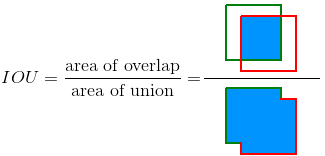
\includegraphics[scale=0.7]{figures/eval_iou.png}
    \end{center}
    \caption[Intersection Over Union metric for object detection]
    {Intersection Over Union metric for object detection,
        the green box represents ground truth and the red box represents
        detection result. The blue area on top represents intersection and
        the one on bottom represents union.}
    \label{fig:eval-iou}
\end{figure}

With the computed $\mathit{IOU}$ result and a hyper-parameter
$\mathit{threshold}$ which usually set to $50\%$, $75\%$ or $90\%$,
we can define the following four terms to describe a detection:

\begin{itemize}
    \item True positive, a correct detection where $\mathit{IOU} \geq
    \mathit{threshold}$.
    \item False positive, a incorrect detection where $\mathit{IOU} <
    \mathit{threshold}$.
    \item True negative, does not apply.
    \item False negative, a ground truth not detected.
\end{itemize}

\subsubsection{Precision-Recall Curve}
\label{sec:Eval-pr-curve}

By analyzing these result, there are two metrics precision and recall can be
used to describe how well the model performs in two different aspects.
Precision \autoref{eq:precision} is a fraction of relevant instances among the
retrieved instances which can be used to measures how accurate is your
prediction.
Recall \autoref{eq:recall} is a fraction of relevant instances that have been
retrieved over the total amount of relevant instances which can be used to
measures how good you find all the positives.

\begin{equation}
\label{eq:precision}
\mathit{precision} =
\frac
{\text{\# true positive}}
{\text{\# true positive + \# false positive}}
\end{equation}

\begin{equation}
\label{eq:recall}
\mathit{recall} =
\frac
{\text{\# true positive}}
{\text{\# true positive + \# false negative}}
\end{equation}

%With precision and recall in hand,
%the Precision-Recall curve (P-R curve) is a good way to evaluate the
%performance of an object detector. as the confidence is changed by plotting a
%curve for each object class. An object detector of a particular class is
%considered good if its precision stays high as recall increases, which means
%that if you vary the confidence threshold, the precision and recall will still
%be high. Another way to identify a good object detector is to look for a
%detector that can identify only relevant objects (0 False Positives = high
%precision), finding all ground-truth objects (0 False Negatives = high recall).

With precision and recall in hand, we can construct a Precision-Recall curve
(P-R curve) which will be used to calculate our metric latter. The curve
construction process can be described as the following:

\begin{enumerate}
    \item Collect all the predictions that make for a particular class of
    objects. Rank them in decreasing order according to the confidence score
    given by the model.
    \item  Compare theses predictions with ground truth to see if it is correct
    or not.
    \item Calculate the precision and recall using the given formula for each
    prediction in the ranked list from top to bottom.
\end{enumerate}

%An object detector of a particular class is considered good if its precision
%stays high as recall increases, which means that if you vary the confidence
%threshold, the precision and recall will still be high. Another way to
%identify
%a good object detector is to look for a detector that can identify only
%relevant objects (0 False Positives = high
%precision), finding all ground truth objects (0 False Negatives = high recall).

An example of the P-R curve can be shown as \autoref{fig:eval-pr-curve}, let's
examine how the precision and recall being calculated. The first row of the
right-hand-side table belongs to the prediction whose confidence score is the
highest among all the predictions for a particular class. From the table, we
know that this prediction is true.
Under the assumption total positive results are 5,
according to \autoref{eq:precision} and \autoref{eq:recall},
$precision = \frac{1}{1}=1.0$ and $precision = \frac{1}{5}=0.2$
The third row, with the same pattern. We already have two results (rows) before
so for the this row,
$precision = \frac{2}{3}=0.67$ and $precision = \frac{2}{5}=0.4$.

\begin{figure}
    \centering
    \begin{minipage}[b]{0.65\textwidth}
        \centering
        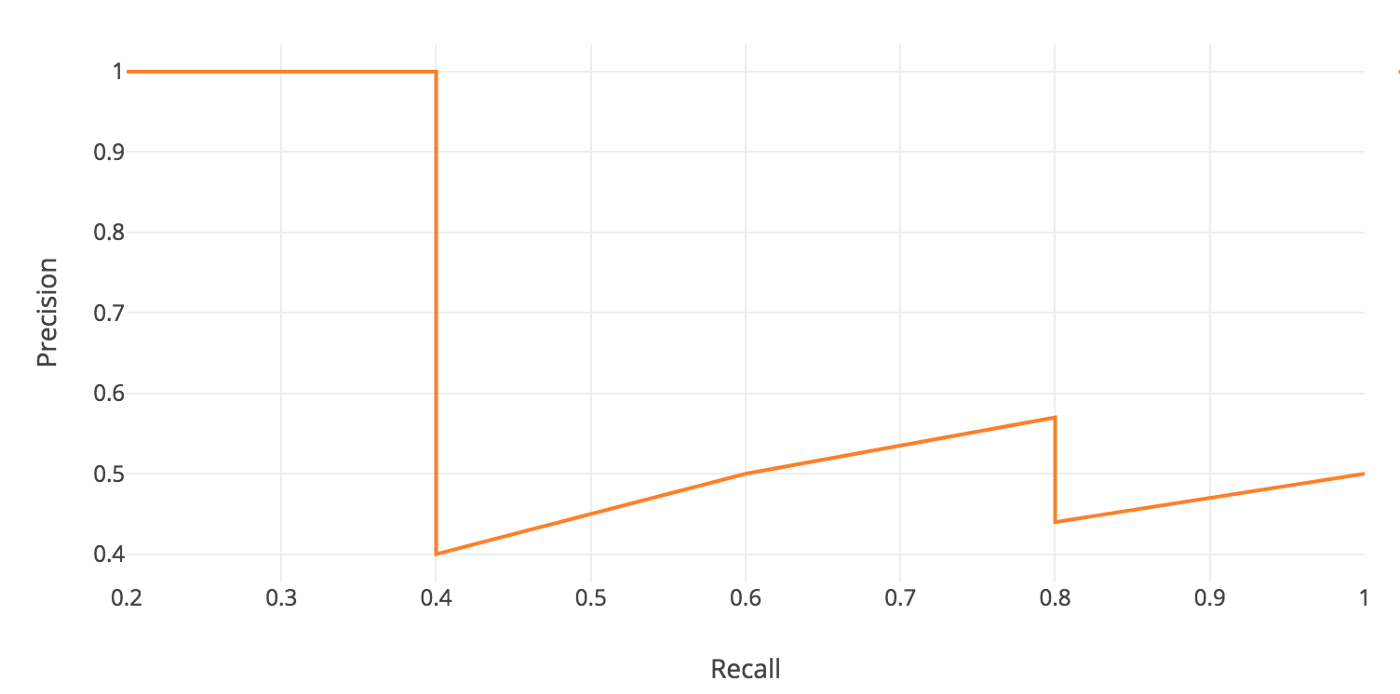
\includegraphics[width=\linewidth]{figures/eval_pr_curve.png}
    \end{minipage}%
    \begin{minipage}[b]{0.35\textwidth}
        \centering
        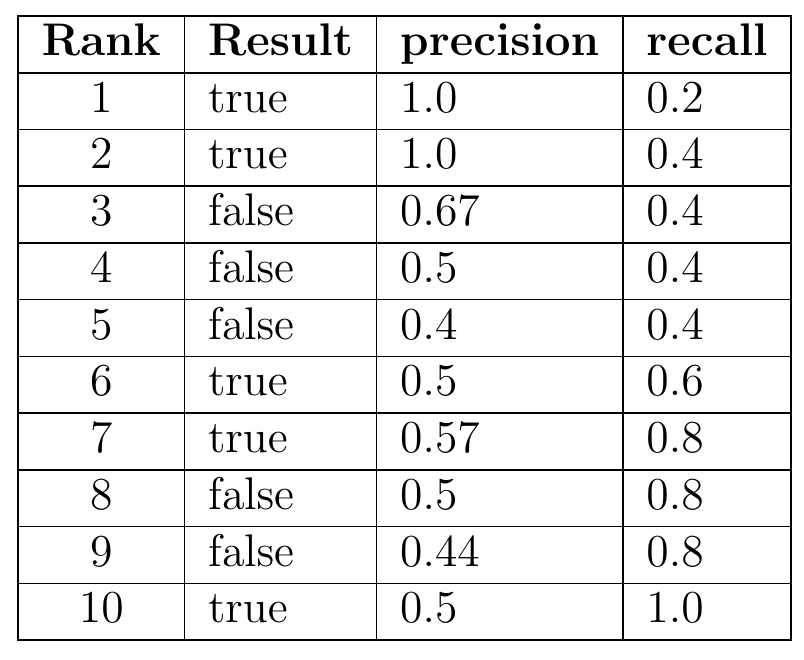
\includegraphics[width=\linewidth]{figures/eval_pr_curve_data.png}
    \end{minipage}
    \caption[An example of Precision-Recall curve]
    {An example of P-R curve, left is the curve itself and right is the data
        used to plot this curve. Assume that there are total five positive
        among
        all these data.}
    \label{fig:eval-pr-curve}
\end{figure}

\subsubsection{Average Precision}
\label{sec:Eval-ap}

Since the P-R curve is often zigzag which is not easy for comparison, an
example can be found on \autoref{fig:eval-pr-curve}, then we may want something
numerical, can be compared directly. Average precision (AP) is such a metric,
in general, it represents the area under the P-R curve and can be formulated as
\autoref{eq:ap}. Precision and recall are always within $[0, 1]$, so to compute
AP we can do integral for the P-R curve within this interval.

\begin{equation}
\label{eq:ap}
\mathit{AP} = \int_0^1p(r)dr
\end{equation}
%
%\begin{figure}
%    \centering
%    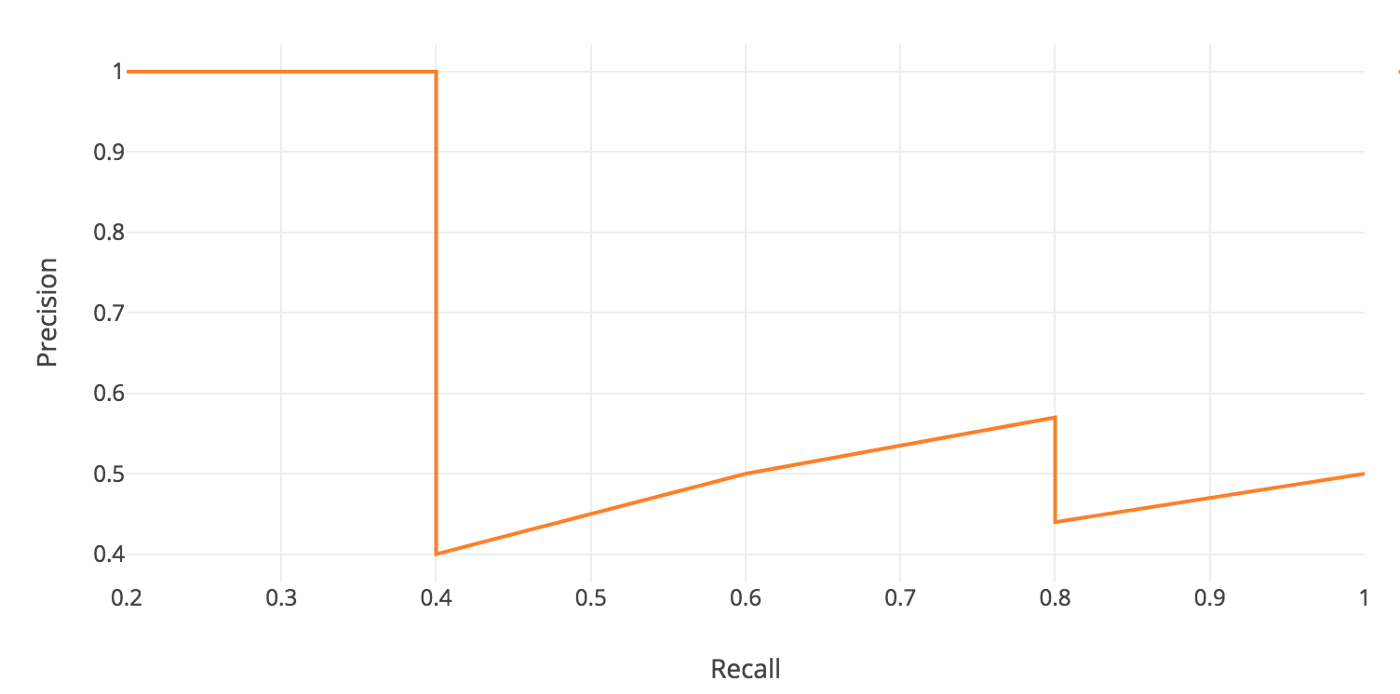
\includegraphics[scale=0.25]{figures/eval_pr_curve.png}
%    \caption{An example of Precision-Recall curve}
%    \label{fig:eval-pr-curve}
%\end{figure}

\begin{figure}
    \begin{center}
        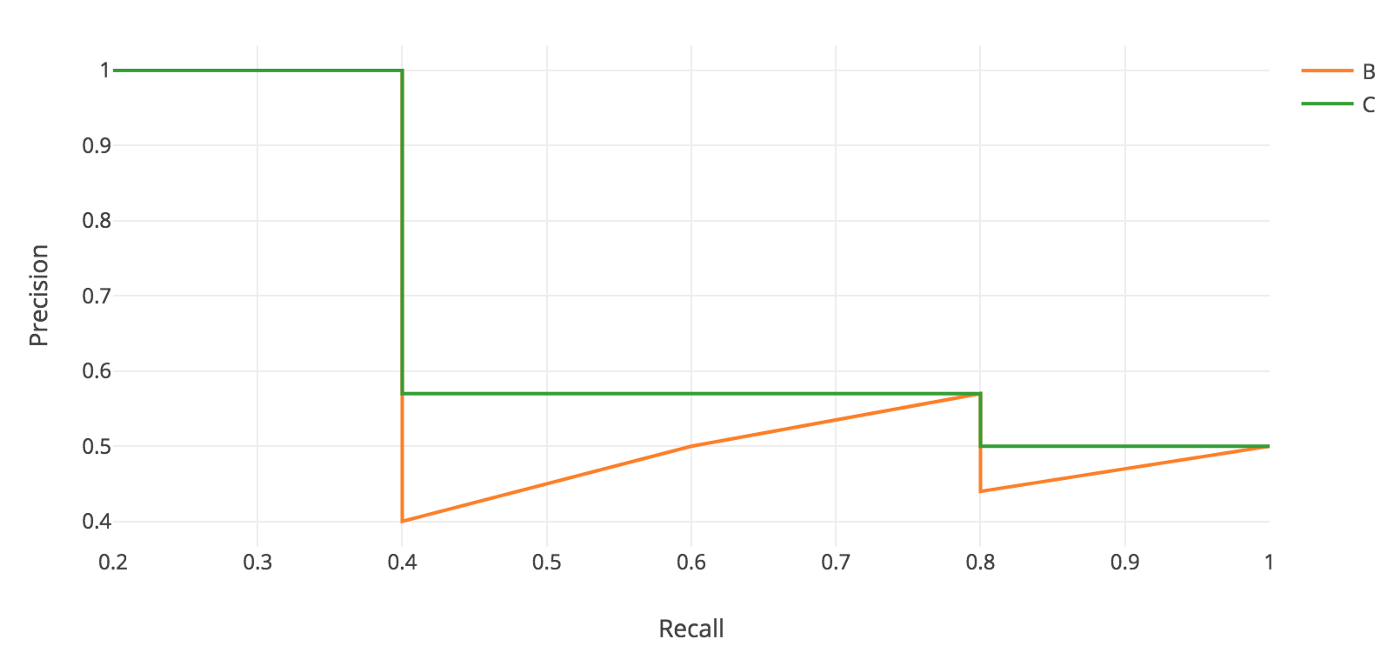
\includegraphics[scale=0.25]{figures/eval_pr_curve2.png}
    \end{center}
    \caption[{An example of smoothed Precision-Recall curve}]
    {An example of smoothed Precision-Recall curve, orange line is the original
        zigzag curve, green line is the smoothed curve}
    \label{fig:eval-pr-curve-2}
\end{figure}

\begin{equation}
\label{eq:smooth-pr-curve}
p_{\text {interp}}(r)=\max _{\widehat{r} \geq r} p(\widetilde{r})
\end{equation}

Under the context of object detection, before we compute AP, for simplicity
purpose we will first smooth the zigzag P-R curve by taking the maximum
precision at each recall level mathematically represents by
\autoref{eq:smooth-pr-curve}.
After smoothing the curve will look like \autoref{fig:eval-pr-curve-2}. Then we
have two kinds of AP: interpolated AP and AP (Area Under Curve, AUC).

\noindent \textbf{Interpolated AP}

\noindent Start from Pascal VOC2008 until VOC2010, an average for the 11-point
interpolated AP is calculated. We firstly divide the recall value into 11 points
$[0.0, 0.1, ..., 1.0]$ then we compute the average of maximum precision value
for these 11 recall values. Precisely, the calculation can be shown by
\autoref{eq:interpl-ap}.

\begin{equation}
\label{eq:interpl-ap}
\begin{aligned} A P &=\frac{1}{11} \sum_{r \in\{0.0, \ldots, 1.0\}} A P_{r} \\
&=\frac{1}{11} \sum_{r \in\{0,0, \ldots, 1,0\}} p_{i n t e r p}(r) \end{aligned}
\end{equation}

\noindent \textbf{AP (Area Under Curve, AUC)}

\noindent For later Pascal VOC2010-2012, all unique recall values are sampled,
whenever the maximum precision value drops. With such operation, we are able to
measure the exact area under the P-R curve after the zigzags are removed. The
operation can be expressed using \autoref{eq:ap-auc}.

\begin{equation}
\label{eq:ap-auc}
\mathrm{AP}=\Sigma\left(r_{n+1}-r_{n}\right) p_{\text
    {imerp}}\left(r_{n+1}\right)
\end{equation}
\noindent where
$$
p_{\text {interp}}
\left(r_{n+1}
\right)=\max _{\tilde{r} \geq r_{n+t}} p(\widetilde{r})
$$

\subsubsection{Experiment Result}
\label{sec:Eval-detection-result}

We trained the YOLO model to become a pedestrian detector using VOC2012 dataset
as explained in \autoref{sec:fw-inst-detector}, then we perform an in-dataset
validation. We randomly sample 5823 images from the dataset as validation set
which never be used for training.
In the randomly sampled validation set, we have total 4372
ground truth boxes. During the validation time, 3950 bounding boxes have been
detected while 3423 of them have been located properly and 527 of them are
the wrong result shown as \autoref{fig:eval-detector-result}. The IOU threshold is
set to 0.5 according to the community's common knowledge.
By performing the detection using our model on the validation set, we have the
Rrecision-Recall curve shown as \autoref{fig:eval-detector-pr}. Since we only
have one class, the mAP will be exactly the person's AP (area under curve)
which is 76.08\% as it is shown on the top of the figure.

For comparison purposes, we used the same model definition training on the same
dataset but with all 20 classes, the result shown as
\autoref{fig:eval-detector-pr1} and \autoref{fig:eval-detector-result1}. The
result obtained from the same sampled validation set. The only difference is the
model used to perform the detection one is the person detection model and the
other is the object detection model with 20 classes supported. We can clearly
find that the result from the object detection model about 5\% outperforms than
that from the person detection model.
That is also explainable since the person detection treats the problem like a
binary classification problem we only train it with person or non-person label
while the object detection model takes it as multi-classes. With a certain amount
of data, a multi-classes detector can perform better than a binary detector.
A straight forward example can be the following. Imagine we have a cat binary classifier
and given a tiger image, the cat classifier may take it as a cat but if we have
another well-trained tiger/cat/dog/fish/etc classifier, then it has a good
chance to classify it properly.

One more thing needs to be mentioned is that in \autoref{sec:fw-inst-detector}
we claim that by theoretical analysis the object detection model should take
more time to train. In our experiment with \texttt{setting 2},
the object detection model takes 504
minutes to train while the person detection model takes 416 minutes to train
unlike our analysis which is one-tenth of its object detection sibling.
That is because we train our model on GPU, with parallel computation
technique supported, it can perform the calculation concurrently.

With the reduction from object detection to person detection, we even lose 5\% 
accuracy. It seems we can only reduce the training time and have nothing to do 
with the inference time, which is actually a bad trade. That's consideration is 
not true. Arguably, if we still use the objection detector, after the detection 
process we may have a large number of bounding boxes being detected. Then we 
need to perform NNS to eliminate those overlapping boxes which is time 
consuming as well as the non-person boxes which is linear time complexity. It
is actually a trade-off between time and accuracy.
Since real-time performance is the hard constraint in our case, we give high
priority to the time instead of accuracy.

\begin{figure}
    \begin{subfigure}
        \centering
        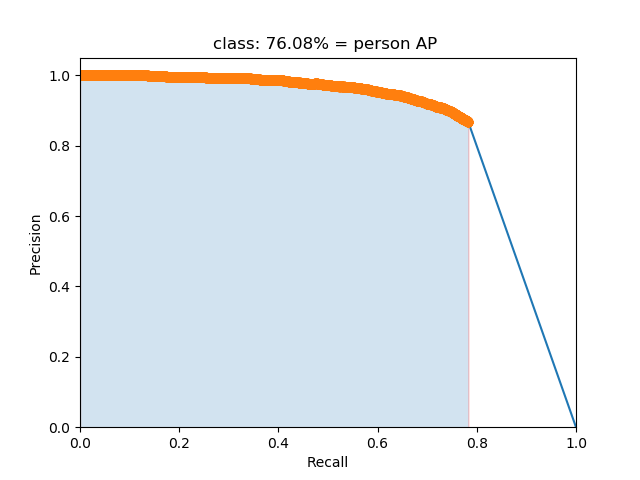
\includegraphics[scale=0.8]{figures/eval_detector_pr_curve.png}
        \caption{Person detection model's Precision-Recall curve on validation
            set.}
        \label{fig:eval-detector-pr}
    \end{subfigure}
    \begin{subfigure}
        \centering
        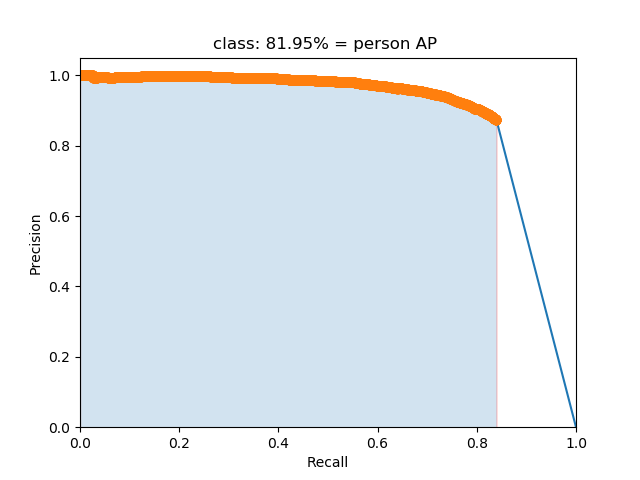
\includegraphics[scale=0.8]{figures/eval_detector_pr_curve1.png}
        \caption{Object detection (with 20 classes supported) model's
            Precision-Recall curve on validation set.}
        \label{fig:eval-detector-pr1}
    \end{subfigure}
\end{figure}

\begin{figure}
    \begin{subfigure}
        \centering
        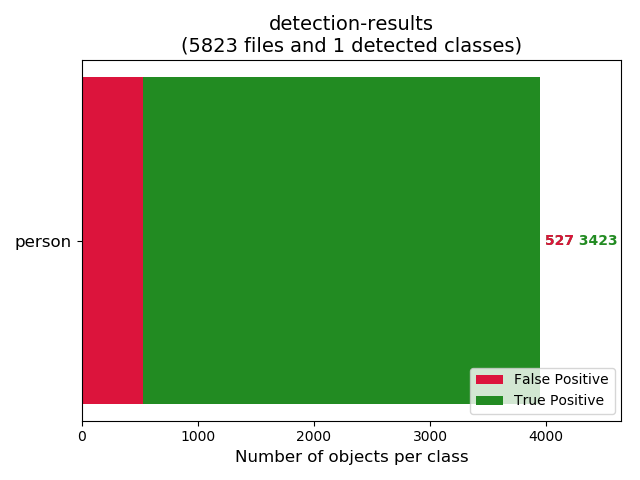
\includegraphics[scale=0.8]{figures/eval_detector_result.png}
        \caption{Person detection result on validation set.}
        \label{fig:eval-detector-result}
    \end{subfigure}
    \begin{subfigure}
        \centering
        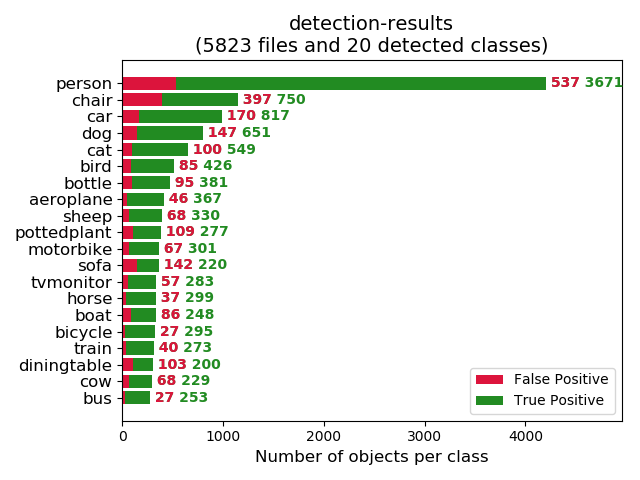
\includegraphics[scale=0.8]{figures/eval_detector_result1.png}
        \caption{Object detection result on validation set.}
        \label{fig:eval-detector-result1}
    \end{subfigure}
\end{figure}

\subsection{Person Retrieval}
\label{sec:Eval-reid}

In the evaluation time, we test our person retrieval implementation described
in \autoref{sec:fw-inst-recoginzer} through the following method:

\begin{enumerate}
    \item We split all the identities we have in the dataset into two parts,
    one is the training set $T$ and the other is validation set $V$. There is no
    overlapping between $T$ and $V$ which means $T \cap V = \emptyset$. Each
    identity has a certain number of images captured from different cameras.

    \item Then we take all the images corresponding to the identities in $V$,
    further splitting them into query set $Q$ and the gallery set $G$. For each
    image in $Q$ there must be at least one corresponding image in $G$ shared
    the same identity label but captured from different cameras.

    \item We use our trained model to extract feature descriptor $f_i^g$ for
    all the images in the gallery to form a database $D$.

    \item For each image $q \in Q$, we also used the same model to extract the
    feature descriptor $f_i^q$, then sort all the descriptors in the database
    according to $\mathit{distance}(f_i^q, f)$ in increasing order.

    \item Find the corresponding identities of the sorted descriptor and return
    them in the same order.
\end{enumerate}

Once have the result, we can take a look into two main metrics for the 
person retrieval task.

\subsubsection{Cumulative Matching Characteristics (CMC)}
\label{sec:Eval-reid-cmc}

Before we discuss cumulative matching characteristics, we would like to explain
two possible settings for the dataset.

\begin{itemize}
    \item Single-galley-shot setting,
    each gallery identify has only one instance (e.g. CUHK03 dataset).

    \item Multi-gallery-shot setting,
    both query and gallery identity have more than one instance in their own
    dataset (e.g. Market1501 dataset).
\end{itemize}

Consider a simple single-gallery-shot setting, for each query, the algorithm
will rand all the gallery images according to their distance to the query in
increasing order, then the CMC top-k accuracy is:

\begin{equation}
\label{eq:cmc}
\mathit{Acc}_{k}=
\left
\{\begin{array}{ll}
{1} & {\text { if top-k ranked gallery samples contain the query identity }} \\
{0} & {\text { otherwise }}
\end{array}
\right.
\end{equation}

\noindent which is a shifted step function. The final CMC curve is computed by
averaging \autoref{eq:cmc} over all the queries.
In this thesis, we applied a new splitting method \cite{dataset-cuhk03-np-2017}
to CUHK03 dataset like the Market1501 and Duke-MTMC dataset did which
originally are multi-gallery-shot setting to ensure the result is comparable.
Under this setting, query and gallery sets could have same camera views, but
for each individual query identity, their gallery samples from the same
camera are excluded.

\subsubsection{Mean Average Precision}
\label{sec:Eval-reid-map}

In order to explain mean average precision (mAP), we will first need to
introduce several related concepts. In the classification problem, we commonly
use the following four terminologies to describe the result (even the name is the
same as the object detection one but the meaning is different here) shown as
\autoref{fig:eval-classif-metric}.

\begin{itemize}
    \item True positive, the model correctly predicts the positive class.
    \item True negative, the model correctly predicts the negative class.
    \item False positive, the model incorrectly predicts the positive class.
    \item False negative, the model incorrectly predicts the negative class.
\end{itemize}

\begin{figure}
    \centering
    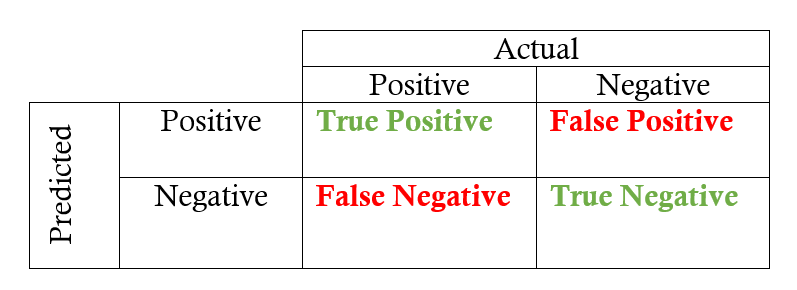
\includegraphics[scale=0.4]{figures/eval_classif_metric.png}
    \caption{Possible result for classification problem.}
    \label{fig:eval-classif-metric}
\end{figure}

Even though the definition of four concepts are various between the objection detection
and ReID tasks. But the formula to calculate precision and recall remain the
same, \autoref{eq:precision} for precision and \autoref{eq:recall} for recall.
%If we plot the precision and recall in the same coordinate, where horizontal
%axis is the recall and the vertical axis is the precision. Then the average
%precision can be defined as the area under the P-R curve which can be
%formulated as \autoref{eq:ap} where $p$ represents precision and $r$
%represents
%recall.
%%
%%\begin{equation}
%%\label{eq:ap}
%%\mathit{AP} = \int_0^1p(r)dr
%%\end{equation}
With the knowledge about P-R curve and AP (AUC) described in
\autoref{sec:Eval-pr-curve} and \autoref{sec:Eval-ap} we can finally give
definition to mean average precision (mAP), it is the mean of average
precision, assume we have $N$ queries during the evaluation time then

\begin{equation}
\label{eq:map}
\mathit{mAP} = \frac{\mathit{AP}}{N} = \dfrac{\int_0^1p(r)dr}{N}
\end{equation}

Apply mAP to evaluate retrieval task firstly proposed in
\cite{dataset-market1501-2015}. The author argued that in multi-gallery-shot
setting, CMC cannot provide a fairly comparison between two rank lists, a
mini-example can be found in \autoref{fig:map-mini-exmaple}. Because that for a ReID
system, we would like to know how accurate the prediction can be, not just the
accuracy among the top $k$ result.

\begin{figure}
    \begin{center}
        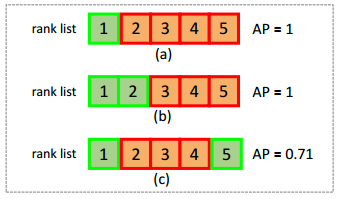
\includegraphics[scale=0.7]{figures/eval_cmc_vs_map.png}
    \end{center}
    \caption[Mini-example for the necessary of AP]
    {Mini-example for the necessary of AP, green box represents a match
        while red box means a mismatch. CMC result for all three cases are
        1, but AP will be [1, 1, 0.71] respectively.}
    \label{fig:map-mini-exmaple}
\end{figure}

\subsubsection{Dataset}
\label{sec:eval-recognizer-dataset}

%Once we defined the network structure, the next step will be training the model
%on the network.
Before we go into our experiment and result, let's take a look at the public
available datasets in this domain. There is a total of three datasets: Market1501
\cite{dataset-market1501-2015}, CUHK03 \cite{dataset-cuhk03-2014} and Duke-MTMC
\cite{dataset-dukemtmc-2016}, which have been employed in our implementation we
are going to introduce, the properties of them shown as
\autoref{tab:reid-dataset}. We provide an abstraction of the dataset
illustrated by \autoref{fig:fw-reid-dataset-uml} and currently encapsulate
these three for our model's training, testing and experiment.

\begin{table}
    \begin{center}
        \begin{tabular}{||c c c c c||}
            \hline
            dataset & subset & \# pids & \# images & \# cameras \\ [0.5ex]
            \hline\hline
            \multirow{3}{4em}{{\tiny Market1501}} & train & 751 & 12936 & 6 \\
            & query & 750 & 3368 & 6 \\
            & gallery & 751 & 15913 & 6 \\
            \hline
            \multirow{3}{4em}{{\tiny CUHK03-NP}} & train & 767 & 7368 & 2 \\
            & query & 700 & 1400 & 2 \\
            & gallery & 700 & 5327 & 2 \\
            \hline
            \multirow{3}{4em}{{\tiny Duke-MTMC}} & train & 702 & 16522 & 8 \\
            & query & 702 & 2228 & 8 \\
            & gallery & 1110 & 17661 & 8 \\
            \hline
        \end{tabular}
    \end{center}
    \caption{Statistic for three popular ReID datasets}
    \label{tab:reid-dataset}
\end{table}

\begin{figure}
    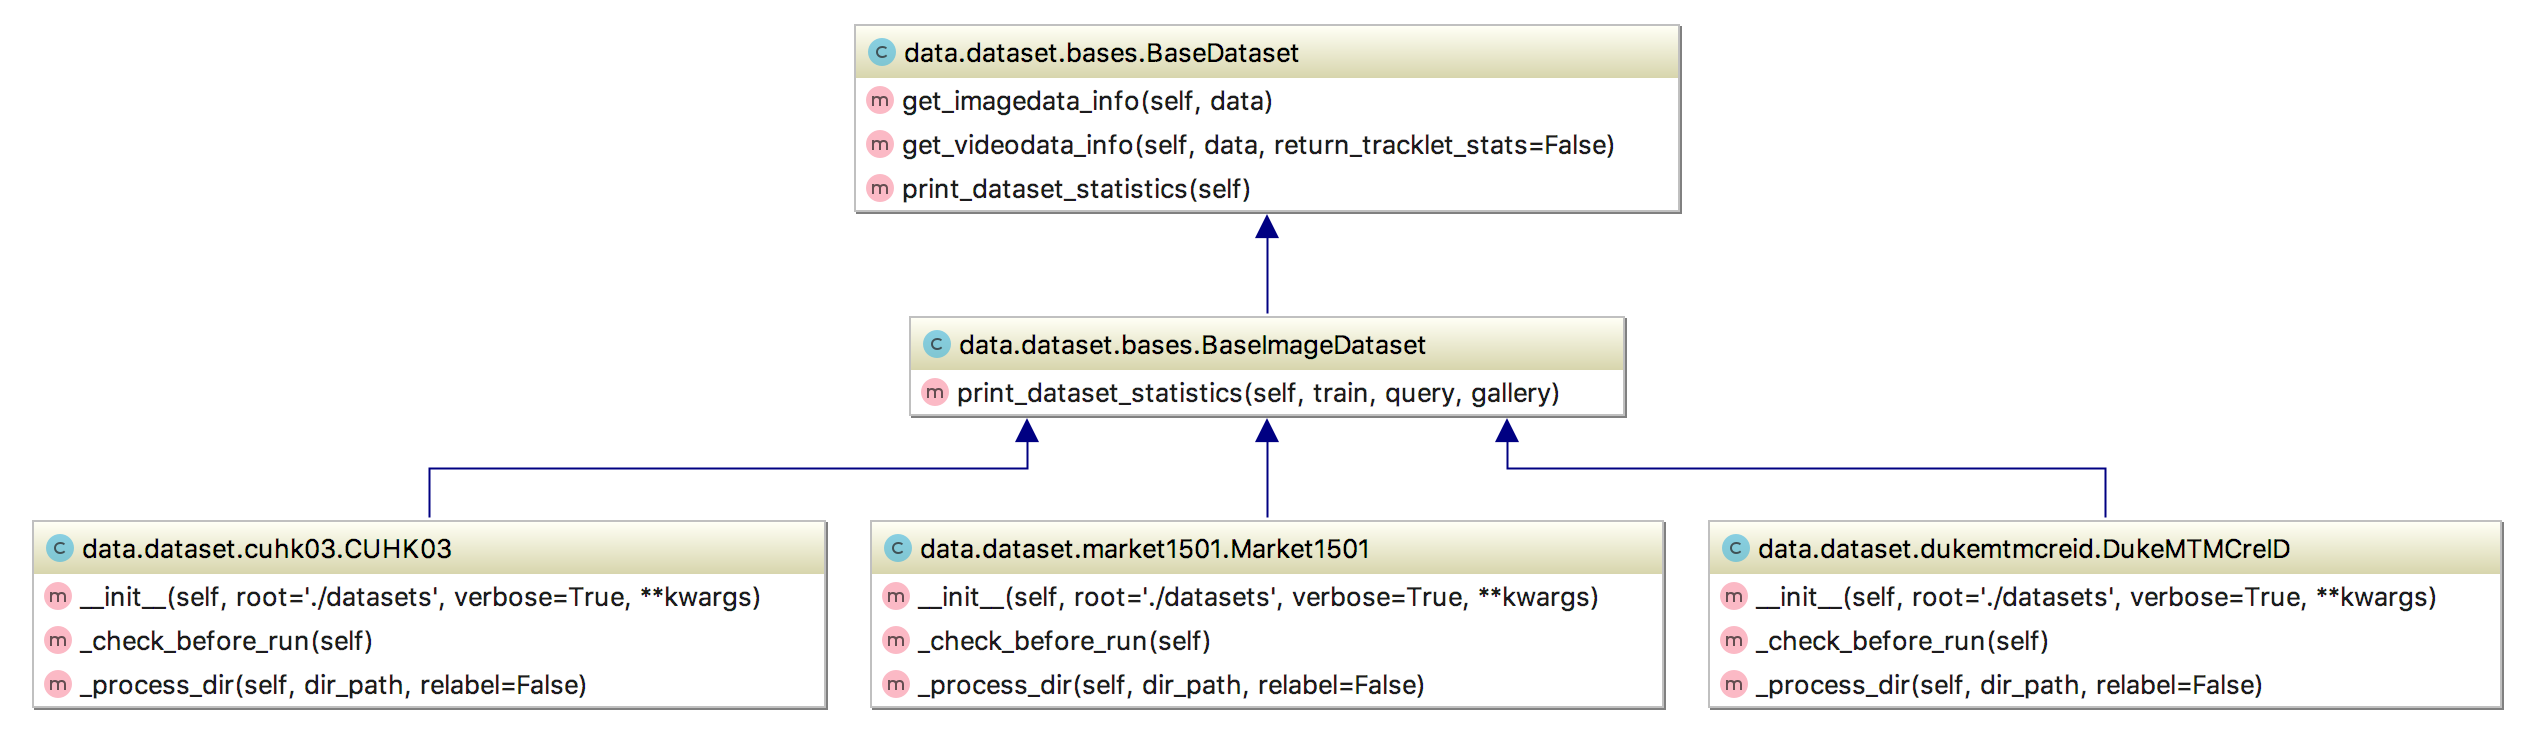
\includegraphics[width=\linewidth]{figures/framework_reid_dataset_uml.png}
    \caption{UML diagrams of ReID dataset abstraction}
    \label{fig:fw-reid-dataset-uml}
\end{figure}

\subsubsection{Experiment Result}
\label{sec:Eval-reid-result}


\begin{table}[]
    \centering
    \begin{tabular}{|l|l|l|l|l|}
        \hline
        \multicolumn{1}{|c|}{\textbf{Rank}} & 
        \multicolumn{1}{c|}{\textbf{Method}} & 
        \multicolumn{1}{c|}{\textbf{CMC}} & 
        \multicolumn{1}{c|}{\textbf{mAP}} & 
        \multicolumn{1}{c|}{\textbf{Year}} \\ \hline
        1 & Auto-ReID & 95.4 & 94.2 & 2019 \\ \hline
        2 & DG-Net(RK) & 95.4 & 92.49 & 2019 \\ \hline
        3 & \begin{tabular}[c]{@{}l@{}}Parameter-Free\\ Spatial 
            Attention\end{tabular} & 94.7 & 91.7 & 2018 \\ \hline
        4 & MGN & 95.7 & 86.9 & 2018 \\ \hline
        6 & DG-Net & 94.8 & 86.0 & 2019 \\ \hline
        6 & OSNet & 94.8 & 84.9 & 2019 \\ \hline
        7 & PCB + RPP & 93.8 & 81.6 & 2017 \\ \hline
        8 & PCB & 92.3 & 77.4 & 2017 \\ \hline
        9 & GLAD* & 89.9 & 73.9 & 2017 \\ \hline
        10 & Incremental Learning & 89.3 & 71.8 & 2018 \\ \hline
    \end{tabular}
    \caption{State of the art result on Market1501 dataset 
    ~\protect\cite{state-of-the-art-market1501}.}
    \label{tab:eval-state-of-art-market1501}
\end{table}

\begin{table}[]
    \centering
    \begin{tabular}{|l|l|l|l|l|}
        \hline
        \multicolumn{1}{|c|}{\textbf{Rank}} & 
        \multicolumn{1}{c|}{\textbf{Method}} & 
        \multicolumn{1}{c|}{\textbf{CMC}} & \multicolumn{1}{c|}{\textbf{mAP}} & 
        \multicolumn{1}{c|}{\textbf{Year}} \\ \hline
        1 & Auto-ReID & 91.4 & 89.2 & 2019 \\ \hline
        2 & DG-Net(RK) & 90.26 & 88.31 & 2019 \\ \hline
        3 & \begin{tabular}[c]{@{}l@{}}Parameter-Free\\ Spatial 
            Attention\end{tabular} & 89.0 & 85.9 & 2018 \\ \hline
        4 & MGN & 88.7 & 78.4 & 2018 \\ \hline
        6 & DG-Net & 86.6 & 74.8 & 2019 \\ \hline
        6 & OSNet & 88.6 & 73.5 & 2019 \\ \hline
        7 & PCB (RPP) & 83.3 & 69.2 & 2017 \\ \hline
        8 & PCB (UP) & 81.8 & 66.1 & 2017 \\ \hline
        9 & SVDNet + Random Erasing & 79.3 & 62.4 & 2017 \\ \hline
        10 & Incremental Learning & 80.0 & 60.2 & 2018 \\ \hline
    \end{tabular}
    \caption{State of the art result on DukeMCMT-reid dataset 
    ~\protect\cite{state-of-the-art-dukemcmt}.}
    \label{tab:eval-state-of-art-dukemcmt}
\end{table}

We perform comprehensive experiments on person re-identification task since it
is the main goal of this thesis, let's walk through them one by one. In order
to give the reader a sense how well our model perform, we provide the state of
the art result obtained from two common datasets shown as
\autoref{tab:eval-state-of-art-market1501} and
\autoref{tab:eval-state-of-art-dukemcmt}. By observing these two tables, we
find that all the results from Market1501 are better than that from
DukeMCMT-reid which indicates the former dataset is in a sense easier than the
latter.

\textbf{Comparison between two different triplet loss functions:}
As mentioned in \cite{in-defense-of-triplet-loss-for-reid-2017}, there are two
kinds of triplet loss functions \autoref{eq:batch-all} and
\autoref{eq:batch-hard}.
We do a comparison between these two losses and train the model with
\texttt{setting 2} on the Market1501 dataset, the validation result we have can
be summarized as \autoref{tab:eval-two-triplet-losses}. Triplet all loss
perform better than triplet hard loss surprisingly, that is in contrast with
the result reported by \cite{in-defense-of-triplet-loss-for-reid-2017}, so far
we don't have a proper explanation for it, our guess is that it may cause by
the implementation where the paper's implementation is in Pytorch and ours is
in TensorFlow.
During the training CMC and mAP metrics, both got improved with time increasing
which perform as our expectation. And the trend becomes more and more stable
when the training time goes up.

\begin{table}[]
    \centering
    \begin{tabular}{|l|r|l|l|}
        \hline
        \textbf{Triplet Loss}                     &
        \multicolumn{1}{c|}{\textbf{Epoch No.}}   &
        \multicolumn{1}{c|}{\textbf{CMC (top 5)}} &
        \multicolumn{1}{c|}{\textbf{mAP}} \\ \hline
        \multicolumn{1}{|c|}{\multirow{3}{*}{triplet all}}
        & 40  & {[}0.808, 0.877, 0.902, 0.902, 0.931{]} & 0.597
        \\ \cline{2-4}
        \multicolumn{1}{|c|}{}
        & 80  & {[}0.898, 0.932, 0.949, 0.962, 0.966{]}  & 0.755
        \\ \cline{2-4}
        \multicolumn{1}{|c|}{}
        & 120 & {[}0.904, 0.941, 0.952, 0.964, 0.969{]} & 0.769
        \\ \hline
        \multirow{3}{*}{triplet hard}
        & 40  & {[}0.803, 0.871, 0.903, 0.920, 0.930{]} & 0.602
        \\ \cline{2-4}
        & 80  & {[}0.868, 0.921, 0.945, 0.955, 0.962{]} & 0.704
        \\ \cline{2-4}
        & 120 & {[}0.878, 0.924, 0.946, 0.955, 0.963{]} & 0.715
        \\ \hline
    \end{tabular}
    \caption[Validation result on the model trained with Market1501 dataset]
    {Validation result on the model trained with Market1501 dataset guided by
        two different loss functions.}
    \label{tab:eval-two-triplet-losses}
\end{table}

\textbf{Comparison between two environment settings:}
We also try to train the model in two different settings in the same Market1501
dataset. And the result can be found by \autoref{tab:eval-two-env}. Obviously,
with the more powerful hardware in \texttt{setting 2}, the training time is
much less than it on \texttt{setting 1}.
%But what surprised us is that the metrics show the result
%we get from \texttt{setting 1} is slightly better than what we obtain from
%\texttt{setting 2}.
Also, as we can see the results obtained from the same loss function are almost
identical the difference is limited to 0.001 which is under expectation, cause
in such a computation task we cannot guarantee the result will be exactly the
same.

\begin{table}[]
    \centering
    \begin{tabular}{|c|c|c|c|}
        \hline
        \textbf{Triplet Loss} & \textbf{Metric} & \textbf{Setting 1} &
        \textbf{Setting 2} \\ \hline
        \multirow{3}{*}{triplet all} & CMC (top 2) & {[}0.904, 0.947{]}
        & {[}0.904, 0.941{]}\\ \cline{2-4}
        & mAP & 0.774 & 0.769 \\ \cline{2-4}
        & \begin{tabular}[c]{@{}c@{}}training time\\ (min)\end{tabular} & 244 &
        133 \\ \hline
        \multirow{3}{*}{triplet hard} & CMC (top 2) & {[}0.871, 0.923{]}
        & {[}0.878, 0.924{]}\\ \cline{2-4}
        & mAP & 0.705 & 0.709 \\ \cline{2-4}
        & \begin{tabular}[c]{@{}c@{}}training time\\ (min)\end{tabular} & 237 &
        134 \\ \hline
    \end{tabular}
    \caption{Training result with two different settings on the same Market1501
    dataset.}
    \label{tab:eval-two-env}
\end{table}

\textbf{Comparison between the result obtained same dataset validation:}
As we mention in \autoref{sec:eval-recognizer-dataset}, we have an abstraction
layer of the ReID dataset which enables us to train on various datasets with
only few modification (actually just pass different parameter).
By making use of it, we perform training and validation on three different
datasets with \texttt{setting 2} and we finally obtain the result shown by
\autoref{tab:eval-dif-datasets}. From the result, we found that the performance
on the CUHK03 dataset is poor, we thought that might due to less of training
samples for the identity from distinct cameras (it has total two cameras
only). And for the other two, since Market1501 is a little be easier than
DukeMTMC-reID dataset so the result we have currently is under expectation.

\begin{table}[]
    \centering
    \begin{tabular}{|r|l|l|}
        \hline
        \textbf{Dataset \textbackslash Metrics} &
        \multicolumn{1}{c|}{\textbf{CMC (top 5)}} &
        \multicolumn{1}{c|}{\textbf{mAP}} \\ \hline
        \textbf{Market1501} & {[}0.904, 0.941, 0.952, 0.964, 0.969{]} & 0.769
        \\ \hline
        \textbf{CUHK03} & {[}0.502, 0.586, 0.641, 0.683, 0.721{]} & 0.500 \\
        \hline
        \textbf{DukeMTMC-reID} & {[}0.840, 0.884, 0.904, 0.919, 0.926{]} &
        0.704 \\ \hline
    \end{tabular}
    \caption{Training and validation result on three different datasets with ID
        and triplet all loss on \texttt{setting 2}.}
    \label{tab:eval-dif-datasets}
\end{table}

\textbf{Comparison between results obtained from cross dataset validation:}
Generalization is used to describe how well a model can handle an unseen style
of data. In order to test the generalization capability of our models, we
perform across dataset validation experiment which means we train the model on
$dataset1$ then test it on $dataset2$. Since we were already known the model
trained with CUHK03 dataset perform poor on this task from the previous
comparison, we don't take it into consideration. The cross dataset validation
result shown as \autoref{tab:eval-cros-datasets} with Market1501 and
DukeMTMC-reID dataset.
From the table, we found that the model trained on DukeMTMC-reID dataset can
obtain a better generalization ability.

\begin{table}[]
    \resizebox{\textwidth}{!}{%
        \begin{tabular}{|r|c|c|}
            \hline
            \multicolumn{1}{|l|}{\textbf{Metrics / Dataset}}
            & \textbf{M $\rightarrow$ D} & \textbf{D $\rightarrow$ M} \\ \hline
            \textbf{CMC} & {[}0.272, 0.339, 0.379, 0.404, 0.420{]} & {[}0.474,
            0.548, 0.587, 0.618, 0.643{]} \\ \hline
            \textbf{mAP} & 0.150 & 0.211 \\ \hline
        \end{tabular}%
    }
    \caption[Cross dataset validation result between Market1501 and
    DukeMTMC-reID dataset on \texttt{setting 2}]
    {Cross dataset validation result between Market1501 and DukeMTMC-reID
        dataset on \texttt{setting 2}. M $\rightarrow$ D represents the model
        trained on Market1501 dataset and tested on DukeMTMC-reID dataset.}
    \label{tab:eval-cros-datasets}
\end{table}

\section{Summary}

In this chapter, we described the evaluation methods we employed to examine the
framework solution we proposed in \autoref{chap:fw-design} and
\autoref{chap:fw-inst}. We first evaluated our two main models for person
detection and person retrieval respectively with commonly used metrics in their
domain, then we examined our framework by showing cases to prove it meet the
requirements we proposed in \autoref{sec:intro-scen-req}.
In the next chapter, we will summarize our work, acknowledge the limitation we
have and point out some potential research paths that can be done in the future.

% EOF
